\documentclass[14pt]{beamer}

\usepackage[english]{babel}

\usepackage[latin1]{inputenc}

\usepackage[T1]{fontenc}

\usepackage{amsmath}
\usepackage{amsfonts}
\usepackage{amssymb}
\usepackage{amsthm}

%\usepackage{tgtermes}
\usepackage{tgheros}
%\usepackage{cmbright}
\usepackage{qtxmath}
%\usepackage{kpfonts}
%\renewcommand{\ttdefault}{txtt}

%\usepackage[amsmath,thmmarks]{ntheorem}

\usepackage{wasysym}

\usepackage{graphics}
\usepackage{url}
\usepackage{listings}
\lstset{
  numbers=none,
  basicstyle=\footnotesize\ttfamily,
  xleftmargin=1em,
  xrightmargin=0em,
  aboveskip=1em,
  belowskip=1em
}

\usepackage{tikz}
\usetikzlibrary{shapes,snakes,positioning}

\tikzstyle{mybox} = [draw=red, fill=blue!20, very thick,
    rectangle, rounded corners, inner sep=10pt, inner ysep=12pt]
\tikzstyle{fancytitle} = [fill=red, text=white]

\setbeamertemplate{navigation symbols}{}
\setbeamertemplate{headline}{}
\setbeamertemplate{footline}{}
\usetheme{default}
%\usecolortheme[named=red]{structure}


\title{Software Licensing\\
  {\footnotesize and the GPL in combination with closed source software}}

\author{Martijn Vermaat}
\institute{Human Genetics, LUMC}
\date{\small Bioinformatics work discussion, October 25, 2011}


\begin{document}


\frame{\titlepage}


\frame{

  \frametitle{IP law}

  Intellectual property (IP) law:

  \vspace{\baselineskip}

  \begin{itemize}
    \item applies to creations of the mind
    \item spans various fields of law
    \item recognizes exclusive rights
    \item (in some jurisdictions)
  \end{itemize}

}


\frame{

  \frametitle{IP rights}

  IP rights include:
  \begin{itemize}
    \item {\bf copyrights}
    \item {\bf patents}
    \item {\bf trade marks}
    \item database rights
    \item breeder rights
    \item portrait rights
    \item \ldots
  \end{itemize}

}


\frame{

  \frametitle{Copyright}

  A copyright is a set of {\em exclusive} rights that are
  \begin{itemize}
    \item automatic
    \item free
    \item long-lasting
    \item international
  \end{itemize}

  \vspace{\baselineskip}

  Copyright applies to works that are
  \begin{itemize}
    \item the result of creative choices
    \item not copied
  \end{itemize}

}


\frame{

  \frametitle{Copyrighted works}

  Examples of copyrighted works:
  \begin{itemize}
    \item {\bf books}
    \item maps
    \item sheet music
    \item dramatic works
    \item paintings
    \item photographs
    \item architectural drawings
    \item sound recordings
    \item computer programs
  \end{itemize}

}


\frame{

  \frametitle{Copyrights}

  Rights protected by copyright:
  \begin{itemize}
    \item reproduction in various forms
    \item distribution of copies
    \item public performance
    \item communication to the public
    \item translation into other languages
    \item adaptation
  \end{itemize}

}


\frame{

  \frametitle{Licensing}

  All use covered by copyright requires permission

  \vspace{\baselineskip}

  Exclusive rights can be {\em licensed} to others by the copyright owner

}


\frame{

  \frametitle{Software licenses}

  Proprietary licenses

  \vspace{\baselineskip}

  Free and open source licenses

  \begin{itemize}
    \item permissive licenses
    \item copyleft licenses
  \end{itemize}

}


\frame{

  \frametitle{MIT license}

  Permissive license

  \vspace{\baselineskip}

  Similar to 2-clause BSD license

  \vspace{\baselineskip}

  Not public domain!

}


\frame{

  \frametitle{GNU General Public License}

  Copyleft license

  \vspace{\baselineskip}

  Most widely used free software license

  \vspace{\baselineskip}

  Clever use of copyright law

  \vspace{\baselineskip}

  Derivative works of code under the GPL must themselves be under the GPL

}


\frame{

  \frametitle{Derivative works}

  What is a derivative work?

  \vspace{\baselineskip}

  \begin{enumerate}
    \item a modified version of the original program
    \item code that calls the original program via \texttt{fork} and \texttt{exec}
    \item code that is linked with the original program (read: library)
  \end{enumerate}

  \vspace{\baselineskip}

  \uncover<2->{1. yes} $\qquad$ \uncover<3->{2. no} $\qquad$ \uncover<4->{3. maybe}

}


\frame{

  \frametitle{MySQLdb}

  Case study: using MySQL from a Python program

  \vspace{\baselineskip}

  \begin{itemize}
    \item MySQL (client and server) is GPL-licensed
    \item Python MySQLdb library is GPL-licensed
    \item MySQLdb uses libmysql (part of MySQL)
    \item MySQLdb is linked {\em dynamically}
  \end{itemize}

}


\frame{

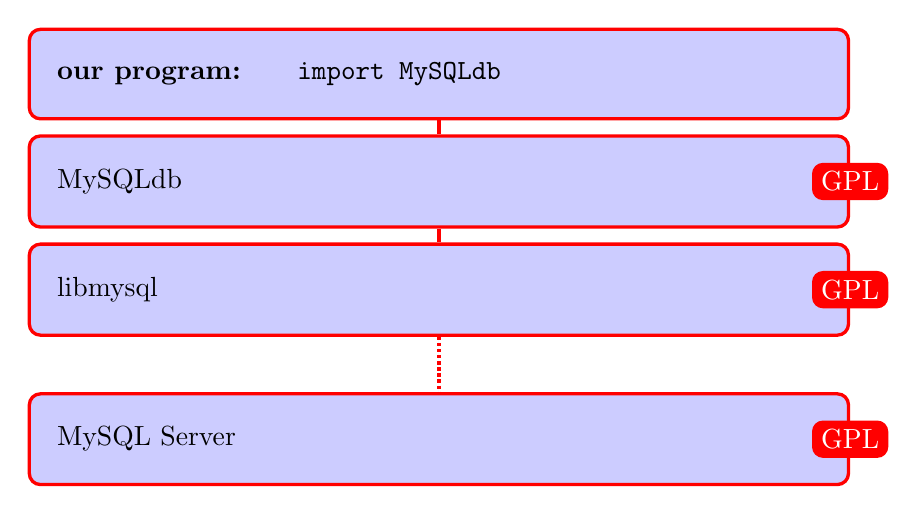
\begin{tikzpicture}

\node [mybox] (box1){%
    \begin{minipage}{0.80\linewidth}
      {\bf our program: $\quad$ \texttt{import MySQLdb}}
    \end{minipage}
};

\node [mybox,below=5pt of box1.south] (box2) {%
    \begin{minipage}[t!]{0.8\linewidth}
      MySQLdb
    \end{minipage}
    };
\node[fancytitle, rounded corners] at (box2.east) {GPL};

\draw [mybox] (box1) -- (box2);

\node [mybox,below=5pt of box2.south] (box3) {%
    \begin{minipage}[t!]{0.8\linewidth}
      libmysql
    \end{minipage}
    };
\node[fancytitle, rounded corners] at (box3.east) {GPL};

\draw [mybox] (box2) -- (box3);

\node [mybox,below=20pt of box3.south] (box4) {%
    \begin{minipage}[t!]{0.8\linewidth}
      MySQL Server
    \end{minipage}
    };
\node[fancytitle, rounded corners] at (box4.east) {GPL};

\draw[style=densely dotted] [mybox] (box3) -- (box4);

\end{tikzpicture}

}


\frame{

  \frametitle{MySQLdb license}

  Is it really GPL-licensed?

  \begin{itemize}
    \item Most Linux distributions say GPL
    \item SF project page says ``GNU General Public License
      (GPL), Python License (CNRI Python License), Zope Public License''
    \item Source code says ``GPL or the original license based on Python
      1.5.2's license''
  \end{itemize}

  The Python 1.5.2 license is an MIT-like license ({\em not} the CNRI
  Python License)

}


\frame{

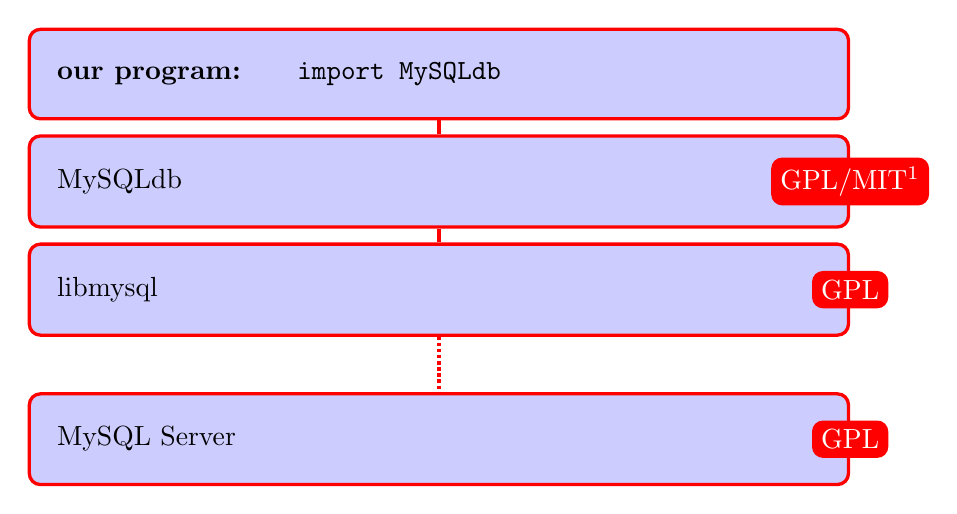
\begin{tikzpicture}

\node [mybox] (box1){%
    \begin{minipage}{0.80\linewidth}
      {\bf our program: $\quad$ \texttt{import MySQLdb}}
    \end{minipage}
};

\node [mybox,below=5pt of box1.south] (box2) {%
    \begin{minipage}[t!]{0.8\linewidth}
      MySQLdb
    \end{minipage}
    };
\node[fancytitle, rounded corners] at (box2.east) {GPL/MIT$^1$};

\draw [mybox] (box1) -- (box2);

\node [mybox,below=5pt of box2.south] (box3) {%
    \begin{minipage}[t!]{0.8\linewidth}
      libmysql
    \end{minipage}
    };
\node[fancytitle, rounded corners] at (box3.east) {GPL};

\draw [mybox] (box2) -- (box3);

\node [mybox,below=20pt of box3.south] (box4) {%
    \begin{minipage}[t!]{0.8\linewidth}
      MySQL Server
    \end{minipage}
    };
\node[fancytitle, rounded corners] at (box4.east) {GPL};

\draw[style=densely dotted] [mybox] (box3) -- (box4);

\end{tikzpicture}

\vspace{\baselineskip}

$^1$ dual-licensed

}


\frame{

  \frametitle{GPL violation?}

  \begin{enumerate}
    \item MySQLdb licensed under MIT-like license
    \item MySQLdb links to libmysql (GPL-licensed)
  \end{enumerate}

  \vspace{\baselineskip}

  1 + 2 = GPL violation

}


\frame{

  \frametitle{libmysql}

  MySQL FLOSS License Exception

  \vspace{\baselineskip}

  Included as file \texttt{EXCEPTIONS-CLIENT}

  \vspace{\baselineskip}

  Rationale:
  \begin{quote}
    We want specified [open source software] to be able to
    use specified GPL-licensed MySQL client libraries [\ldots]
  \end{quote}

}


\frame{

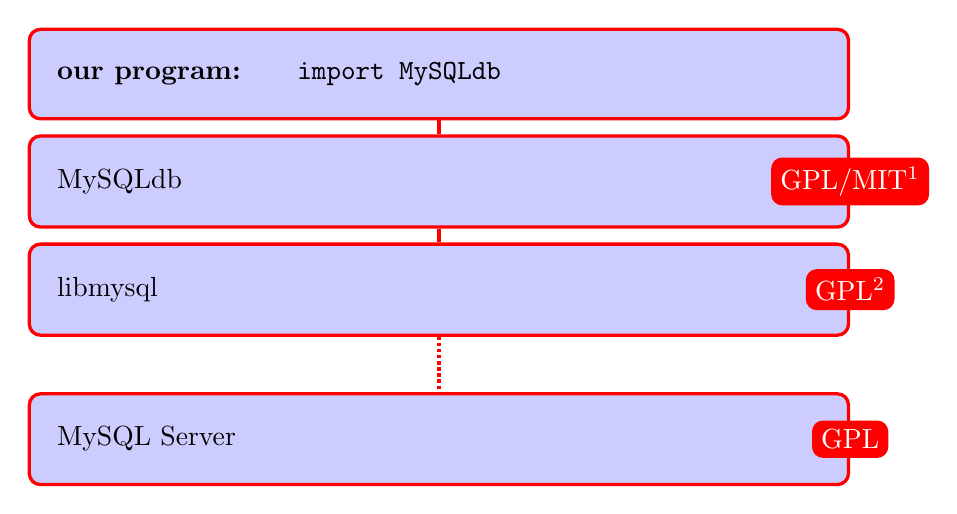
\begin{tikzpicture}

\node [mybox] (box1){%
    \begin{minipage}{0.80\linewidth}
      {\bf our program: $\quad$ \texttt{import MySQLdb}}
    \end{minipage}
};

\node [mybox,below=5pt of box1.south] (box2) {%
    \begin{minipage}[t!]{0.8\linewidth}
      MySQLdb
    \end{minipage}
    };
\node[fancytitle, rounded corners] at (box2.east) {GPL/MIT$^1$};

\draw [mybox] (box1) -- (box2);

\node [mybox,below=5pt of box2.south] (box3) {%
    \begin{minipage}[t!]{0.8\linewidth}
      libmysql
    \end{minipage}
    };
\node[fancytitle, rounded corners] at (box3.east) {GPL$^2$};

\draw [mybox] (box2) -- (box3);

\node [mybox,below=20pt of box3.south] (box4) {%
    \begin{minipage}[t!]{0.8\linewidth}
      MySQL Server
    \end{minipage}
    };
\node[fancytitle, rounded corners] at (box4.east) {GPL};

\draw[style=densely dotted] [mybox] (box3) -- (box4);

\end{tikzpicture}

\vspace{\baselineskip}

$^1$ dual-licensed\\
$^2$ with client exception

}


\frame{

  \frametitle{PEP 249}

  MySQLdb implements PEP 249 (Python Database API spec)

  \vspace{\baselineskip}

  Interchangeable with other implementations

  \vspace{\baselineskip}

  \texttt{import MySQLdb} $\quad \Rightarrow \quad$ \texttt{import drizzle}

}


\frame{

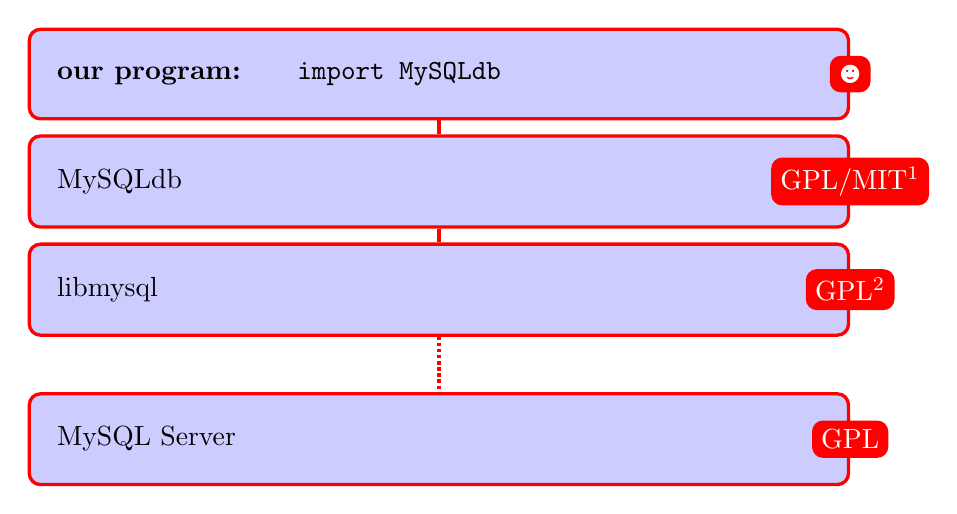
\begin{tikzpicture}

\node [mybox] (box1){%
    \begin{minipage}{0.80\linewidth}
      {\bf our program: $\quad$ \texttt{import MySQLdb}}
    \end{minipage}
};
\node[fancytitle, rounded corners] at (box1.east) {$\blacksmiley$};

\node [mybox,below=5pt of box1.south] (box2) {%
    \begin{minipage}[t!]{0.8\linewidth}
      MySQLdb
    \end{minipage}
    };
\node[fancytitle, rounded corners] at (box2.east) {GPL/MIT$^1$};

\draw [mybox] (box1) -- (box2);

\node [mybox,below=5pt of box2.south] (box3) {%
    \begin{minipage}[t!]{0.8\linewidth}
      libmysql
    \end{minipage}
    };
\node[fancytitle, rounded corners] at (box3.east) {GPL$^2$};

\draw [mybox] (box2) -- (box3);

\node [mybox,below=20pt of box3.south] (box4) {%
    \begin{minipage}[t!]{0.8\linewidth}
      MySQL Server
    \end{minipage}
    };
\node[fancytitle, rounded corners] at (box4.east) {GPL};

\draw[style=densely dotted] [mybox] (box3) -- (box4);

\end{tikzpicture}

\vspace{\baselineskip}

$^1$ dual-licensed\\
$^2$ with client exception

}


\frame{

  \frametitle{Acknowledgements}

  Software Licensing Workshop\\
  {\small NBIC, September 8, 2011}

  \vspace{\baselineskip}

  Maurits Westerik\\
  {\small Bird\&Bird}

  \vspace{\baselineskip}

  Peter Taschner\\
  Ivo Fokkema\\
  Jeroen Laros\\
  {\small Human Genetics, LUMC}

}


\end{document}
